\documentclass{article}
\usepackage[T1]{fontenc}
\usepackage[polish]{babel}
\usepackage[utf8]{inputenc}
\usepackage{amsmath}

\usepackage[margin=1in]{geometry}

\usepackage{listings}
\usepackage{xcolor}
\usepackage{graphicx} 

\definecolor{codegreen}{rgb}{0,0.6,0}
\definecolor{codegray}{rgb}{0.5,0.5,0.5}
\definecolor{codepurple}{rgb}{0.58,0,0.82}
\definecolor{backcolour}{rgb}{0.95,0.95,0.92}

\lstdefinestyle{mystyle}{
    backgroundcolor=\color{backcolour},   
    commentstyle=\color{codegreen},
    keywordstyle=\color{magenta},
    numberstyle=\tiny\color{codegray},
    stringstyle=\color{codepurple},
    basicstyle=\ttfamily\footnotesize,
    breakatwhitespace=false,         
    breaklines=true,                 
    captionpos=b,                    
    keepspaces=true,                 
    numbers=left,                    
    numbersep=5pt,                  
    showspaces=false,                
    showstringspaces=false,
    showtabs=false,                  
    tabsize=2
}

\lstset{style=mystyle}

\title{Iteracyjne metody rozwiązywania równań liniowych}
\author{Peter Nicholson}
\date{May 2020}

\begin{document}

\maketitle

\section{Układy równań}
\(A_1 =\)
\begin{bmatrix}
4 & -1 & -0.2 & 2 \\
-1 & 5 & 0 & -2 \\
0.2 & 1 & 10 & -1 \\
0 & -2 & -1 & 4
\end{bmatrix}
\(B_1 = \)
\begin{bmatrix}
30 \\
0 \\
-10 \\
5
\end{bmatrix}

\noindent
\\
\\
\(A_2 =\)
\begin{bmatrix}
5 & 1 & 1 & 1 \\
1 & 5 & 1 & 1 \\
1 & 1 & 5 & 1 \\
1 & 1 & 1 & 5
\end{bmatrix}
\(B_2 = \)
\begin{bmatrix}
13 \\
16 \\
19 \\
22
\end{bmatrix}

\noindent
\\
\\
\(A_3 =\)
\begin{bmatrix}
4 & -1 & -1 & 0 \\
-1 & 4 & 0 & -1 \\
-1 & 0 & 4 & -1 \\
0 & -1 & -1 & 4
\end{bmatrix}
\(B_3 = \)
\begin{bmatrix}
1 \\
2 \\
0 \\
1
\end{bmatrix}

\noindent
\\
\\
\(A_4 =\)
\begin{bmatrix}
1 & 0.5 & 1 & 0.2 \\ 
0.1 & 3 & 0.2 & 0.4 \\
0.3 & 1 & 2 & 1 \\
1 & 0.5 & 0.2 & 3 \\
\end{bmatrix}
\(B_4 = \)
\begin{bmatrix}
5.2 \\
7.1 \\ 
9.3 \\
5.6 
\end{bmatrix}

\noindent
\\
\\
\(A_5 =\)
\begin{bmatrix}
4 & -2 & 0 \\
-2 & 5 & -2 \\
-2 & 0 & 5
\end{bmatrix}
\(B_5 = \)
\begin{bmatrix}
-6 \\
3 \\
8
\end{bmatrix}

\noindent
\\
\\
\(A_6 =\)
\begin{bmatrix}
60 & 3 & 3 & 3 & 3 & 3 & 3 & 3 \\
3 & 60 & 3 & 3 & 3 & 3 & 3 & 3 \\
3 & 3 & 60 & 3 & 3 & 3 & 3 & 3 \\
3 & 3 & 3 & 60 & 3 & 3 & 3 & 3 \\
3 & 3 & 3 & 3 & 60 & 3 & 3 & 3 \\ 
3 & 3 & 3 & 3 & 3 & 60 & 3 & 3 \\
3 & 3 & 3 & 3 & 3 & 3 & 60 & 3 \\ 
3 & 3 & 3 & 3 & 3 & 3 & 3 & 60
\end{bmatrix}
\(B_6 = \)
\begin{bmatrix}
20 \\
22 \\
24 \\
26 \\ 
28 \\ 
30 \\ 
32 \\
34
\end{bmatrix}

\clearpage

\section{Metoda Jacobiego}

Metodę Jacobiego można wykorzystać, gdy macierz \emph{A} jest dominująca (tzn. suma wartości nie leżących na przekątej w danym wierszu jest mniejsza bądź równa od wartości bezwzględej wartości na przekątnej). To samo tyczy się kolejnych metod.
Macierz kolumnowa \emph{x} w k-tej iteracji ma postać:
\[x_{{k+1}}\,=D^{{-1}}(b-(L+U)x_{{k}})\]
Gdzie \emph{D}, \emph{L}, \emph{U} to odpowiednio macierz diagonalna, trójkątna dolna, trójkątna górna składająca się z odpowiednich wartości macierzy \emph{A}. Ostatecznie \(x_i\) w \emph{k}-tej iteracji ma postać:
\[x^{{(k+1)}}_{i}=\frac{1}{a_{{ii}}}\left(b_{i}-\sum _{{j\neq i}}a_{{ij}}x^{{(k)}}_{j}\right)\]



\begin{lstlisting}[language=C++]
std::vector<double> jacobi(int n, int iter_count, std::vector<std::vector<double>> a, std::vector<double> b) {
    std::vector<double> x(n, 0);

    for (int k = 0; k < iter_count; k++) {
        std::vector<double> x_tmp(n, 0);

        for (int i = 0; i < n; i++) {
            double s = 0;
            for (int j = 0; j < n; j++) {
                if (j != i) s += a[i][j] * x[j];
            }

            x_tmp[i] = (1.0 / a[i][i]) * (b[i] - s); 
        }

        x = x_tmp;
    }

    return x;
}
\end{lstlisting}
Zmienna \emph{iter\_count} określa ilość iteracji. Innym sposobem na zakończenie iteracyjnego wyznaczania rozwiązania byłoby sprawdzenie, czy zmiana wyznaczonych wartości w porównaniu do poprzedniej iteracji jest mniejsza od jakiegoś z góry ustalonego parametru \(\epsilon\).
Błąd (dokładność) rozwiązania w danej iteracji obliczam jako średnią różnic bezwględnych dla każdego x-a. Wyznaczone wartości (w 30 iteracjach):

\noindent
\\
\\
\(X_1 = \)
\begin{bmatrix}
6.9615 \\
2.22118 \\
-1.15413 \\
2.07198
\end{bmatrix}
\(X_2 = \)
\begin{bmatrix}
1.0625 \\
1.8125 \\
2.5625 \\
3.3125
\end{bmatrix}
\(X_3 = \)
\begin{bmatrix}
0.5 \\
0.75 \\
0.25 \\
0.5 
\end{bmatrix}
\(X_4 = \)
\begin{bmatrix}
0.9953 \\
1.9991 \\
2.9971 \\
0.9976 
\end{bmatrix}
\(X_5 = \)
\begin{bmatrix}
-1.2222 \\
0.5555 \\
1.1111
\end{bmatrix}
\(X_6 = \)
\begin{bmatrix}
0.2105 \\
0.2456 \\
0.2807 \\
0.3157 \\
0.3508 \\
0.3859 \\
0.4210 \\
0.4561
\end{bmatrix}

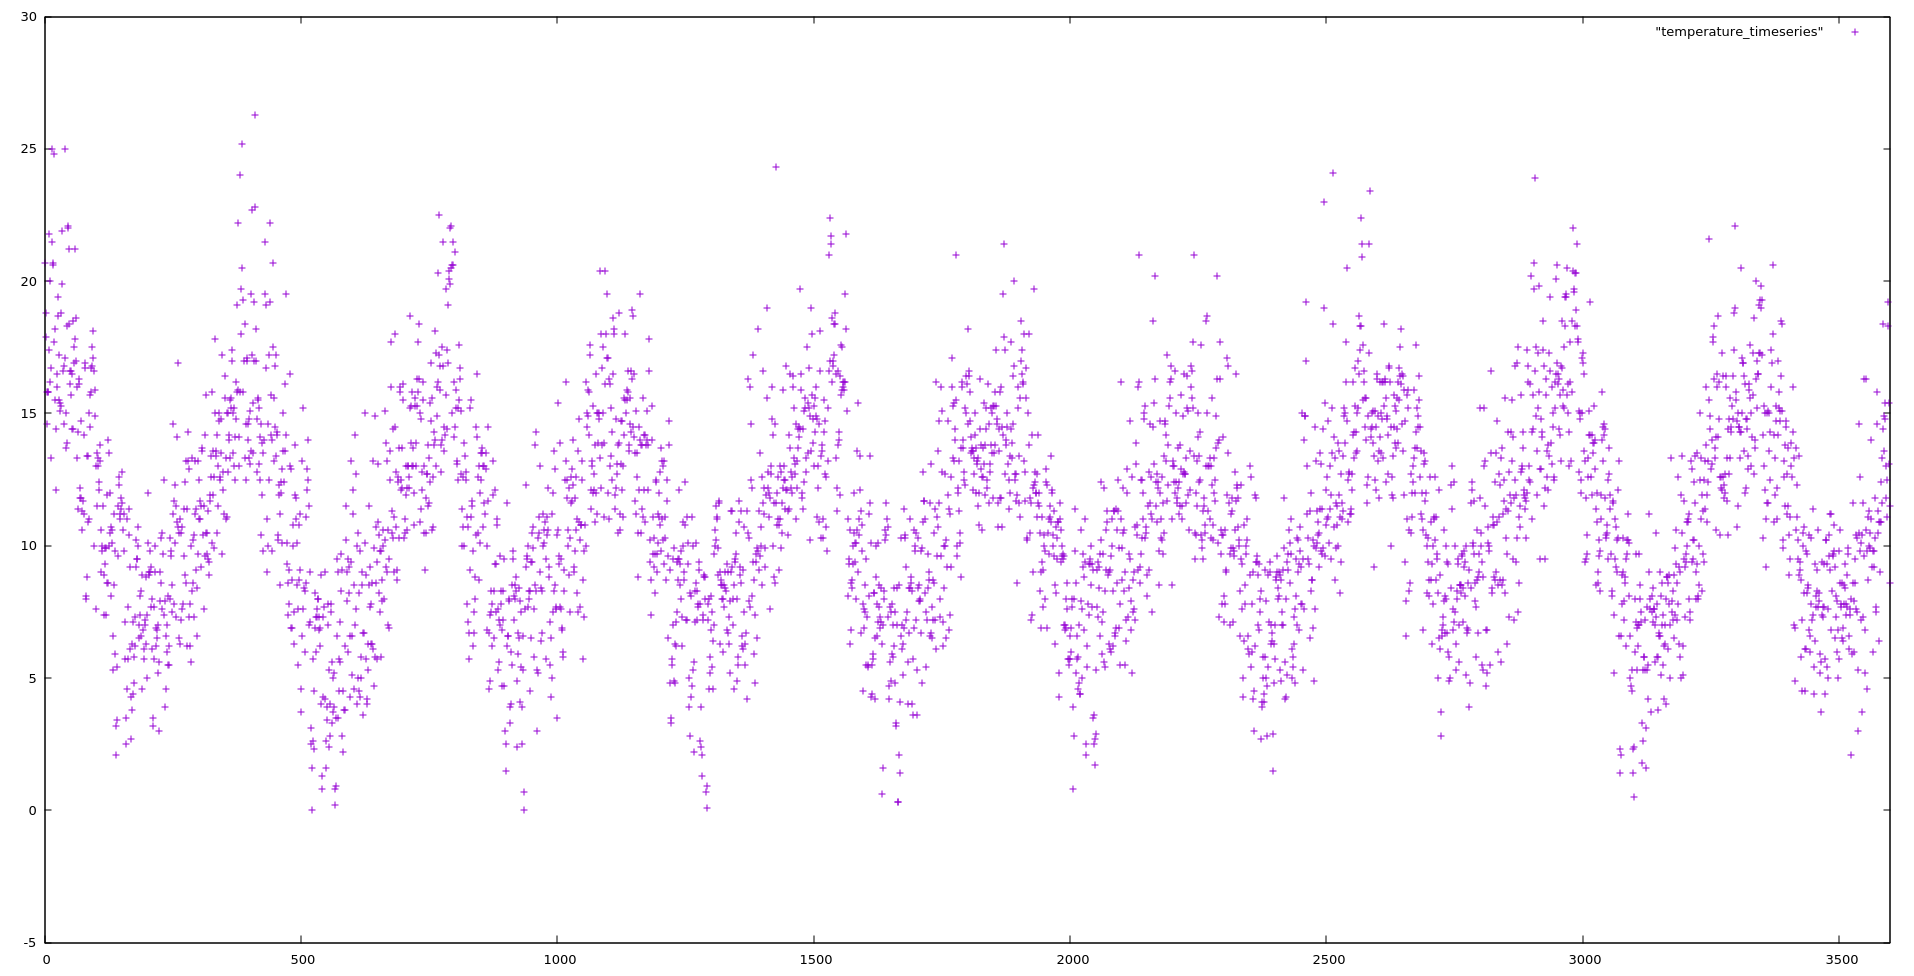
\includegraphics{images/plot1.png}
\clearpage

\section{Metoda Gaussa-Seidela}

W tej metodzie postępujemy podobnie jak w metodzie Jacobiego, z tą różnicą, że w danej iteracji bierzemy pod uwagę wartości \(x_i\) policzone w danej iteracji (jeżeli zostały już policzone) oraz w poprzedniej iteracji. Otrzymujemy zależność:
\[x^{{(k+1)}}_{i}=\frac{1}{a_{{ii}}}\left(b_{i}-\sum _{{j<i}}a_{{ij}}x^{{(k+1)}}_{j}-\sum _{{j>i}}a_{{ij}}x^{{(k)}}_{j}\right)\]

\begin{lstlisting}[language=C++]
std::vector<double> gs(int n, int iter_count, std::vector<std::vector<double>> a, std::vector<double> b) {
    std::vector<double> x(n, 0);

    for (int k = 0; k < iter_count; k++) {
        std::vector<double> x_tmp(n, 0);

        for (int i = 0; i < n; i++) {
            double s1 = 0, s2 = 0;
            
            for (int j = 0; j < i; j++) {
                s1 += a[i][j] * x_tmp[j];
            }

            for (int j = i + 1; j < n; j++) {
                s2 += a[i][j] * x[j];
            }

            x_tmp[i] = (1.0 / a[i][i]) * (b[i] - s1 - s2); 
        }

        x = x_tmp;
    }

    return x;
}
\end{lstlisting}
Wyznaczone wartości (w 30 iteracjach):
\noindent
\\
\\
\(X_1 = \)
\begin{bmatrix}
6.96156 \\ 
2.22112 \\
-1.15414 \\
2.07203
\end{bmatrix}
\(X_2 = \)
\begin{bmatrix}
1.0625 \\
1.8125 \\
2.5625 \\
3.3125 
\end{bmatrix}
\(X_3 = \)
\begin{bmatrix}
0.5 \\
0.75 \\
0.25 \\
0.5 
\end{bmatrix}
\(X_4 = \)
\begin{bmatrix}
1 \\
2 \\
3 \\
1 
\end{bmatrix}
\(X_5 = \)
\begin{bmatrix}
-1.2222 \\
0.5555 \\
1.1111
\end{bmatrix}
\(X_6 = \)
\begin{bmatrix}
0.2105 \\
0.2456 \\
0.2807 \\
0.3157 \\
0.3508 \\
0.3859 \\
0.4210 \\
0.4561
\end{bmatrix}

\clearpage

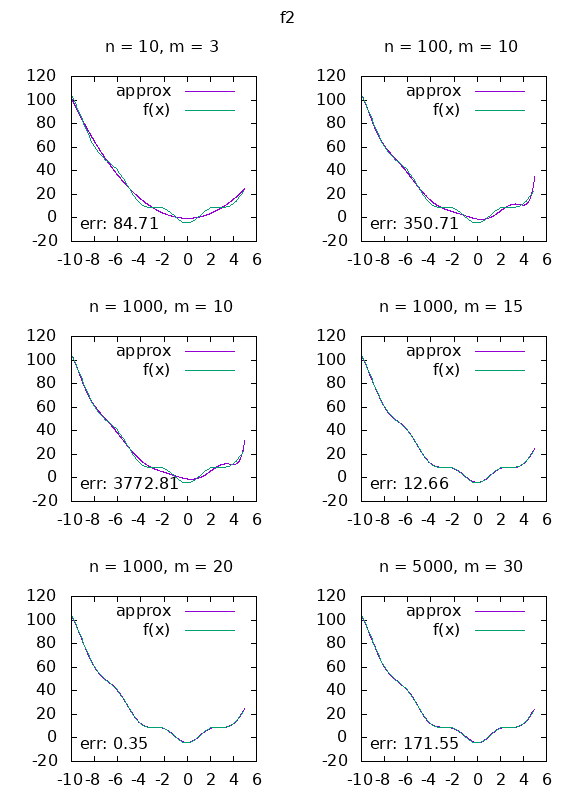
\includegraphics{images/plot2.png}
\clearpage

\section{Successive over-relaxation}
Metoda SOR polega na przyspieszeniu metody Gaussa-Seidela poprzez wprowadzenie parametru relaksacji \(\omega\). Wtedy kolejne przybliżenia wartości \(x_i\) wyznaczamy jako kombinację poprzedniego przybliżenia i przybliżenia wyznaczonego w danej iteracji. Otrzymujemy wzór:
\[x_{i}^{(k+1)}=(1-\omega )x_{i}^{(k)}+{\frac {\omega }{a_{ii}}}\left(b_{i}-\sum _{j\lt i}a_{ij}x_{j}^{(k+1)}-\sum _{j\gt i}a_{ij}x_{j}^{(k)}\right)\]

\begin{lstlisting}[language=C++]
std::vector<double> sor(int n, int iter_count, double w, std::vector<std::vector<double>> a, std::vector<double> b) {
    std::vector<double> x(n, 0);

    for (int k = 0; k < iter_count; k++) {
        std::vector<double> x_tmp(n, 0);

        for (int i = 0; i < n; i++) {
            double s1 = 0, s2 = 0;
            
            for (int j = 0; j < i; j++) {
                s1 += a[i][j] * x_tmp[j];
            }

            for (int j = i + 1; j < n; j++) {
                s2 += a[i][j] * x[j];
            }

            x_tmp[i] = (1 - w) * x[i] + (w / a[i][i]) * (b[i] - s1 - s2); 
        }

        x = x_tmp;
    }

    return x;
}
\end{lstlisting}
Wyznaczone wartości (w 30 iteracjach, dla \(\omega = 0.5\) i \(\omega = 1.1 \)):
\noindent
\\
\\
\(X_1 = \)
\begin{bmatrix}
6.96156 \\ 
2.22112 \\
-1.15414 \\
2.07203
\end{bmatrix}
\(X_2 = \)
\begin{bmatrix}
1.0625 \\
1.8125 \\
2.5625 \\
3.3125 
\end{bmatrix}
\(X_3 = \)
\begin{bmatrix}
0.5 \\
0.75 \\
0.25 \\
0.5 
\end{bmatrix}
\(X_4 = \)
\begin{bmatrix}
1 \\
2 \\
3 \\
1 
\end{bmatrix}
\(X_5 = \)
\begin{bmatrix}
-1.2222 \\
0.5555 \\
1.1111
\end{bmatrix}
\(X_6 = \)
\begin{bmatrix}
0.2105 \\
0.2456 \\
0.2807 \\
0.3157 \\
0.3508 \\
0.3859 \\
0.4210 \\
0.4561
\end{bmatrix}


\clearpage

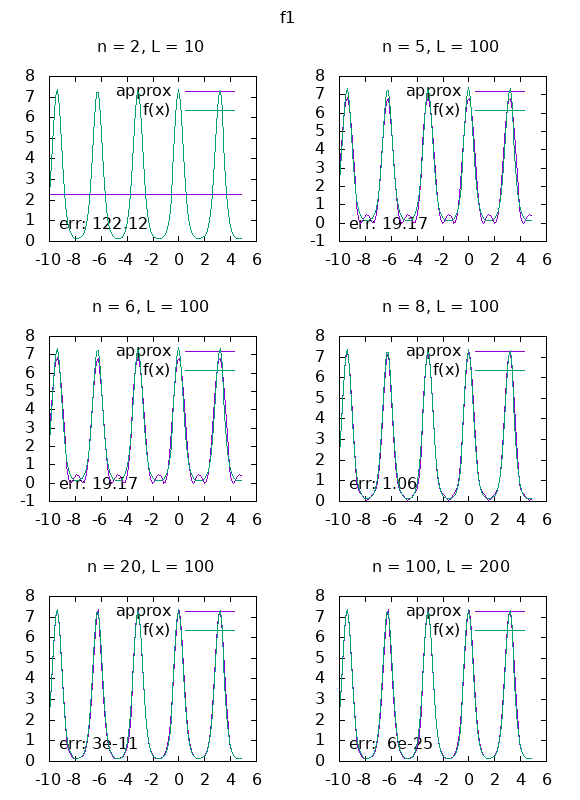
\includegraphics{images/plot3.png}

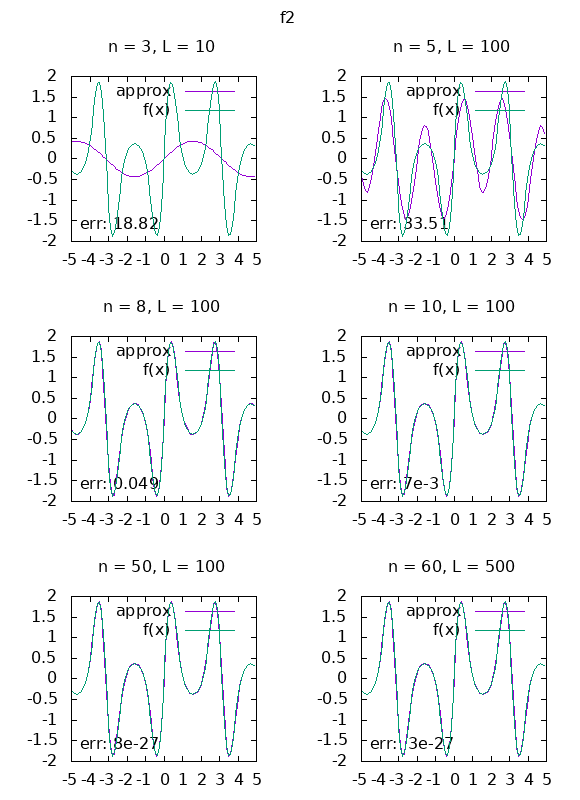
\includegraphics{images/plot4.png}

\clearpage

\section{Porównanie metod}
Metoda Jacobiego jest najprostszą z przedstawionych metod iteracyjnych, lecz charakteryzuje się najgorszą zbieżnością (wymagana jest większa ilość iteracji aby osiągnąć mniejszy błąd). Metoda Gaussa-Seidela modyfikuje metodę Jacobiego poprzez branie pod uwagę przybliżonych wartości obliczonych w danej iteracji, co sprawia, że zbieżność do rozwiązania jest szybsza (osiągana jest w mniejszej liczbie iteracji). Metoda SOR dodatkowo wprowadza parametr relaksacji \(\omega\) który wpływa na prędkość zbiegania do rozwiązania. Wybór parametru relaksacji zazwyczaj jest uzależniony od właściwości macierzy \emph{A}. Dla dobrze wybranej wartości parametru \(\omega\) metoda SOR osiąga najlepszą zbieżność. Zbieżność poszczególnych metod można zaobserwować na przedstawionych wykresach.

\end{document}
